\documentclass{article}

\usepackage{minted}
\usepackage{xcolor}
\usemintedstyle{vs}
\usepackage[utf8]{inputenc}
\usepackage{supertabular}
\usepackage[T1]{fontenc}
\usepackage{icomma}
\usepackage{array} 
\usepackage{color}
\usepackage{amsmath,mathtools}
\usepackage{amssymb,amsfonts}
\usepackage{esint}
\usepackage{multirow}
\usepackage{float}
\usepackage{graphicx}
\usepackage{tikz}
\usepackage[left=2.5cm,right=2.5cm,top=3cm,bottom=3cm]{geometry}
\usepackage{hyperref}
\usepackage[english]{babel}
\usepackage{caption}
\usepackage[bottom]{footmisc}
\usepackage{gensymb}
\usepackage{tabulary}
\usepackage{fancyhdr}
\usepackage{siunitx}
\usepackage{textcomp}
\usepackage[RPvoltages]{circuitikz}
\newcommand{\HRule}{\rule{\linewidth}{0.5mm}}
\usepackage{parskip}
\setlength{\parindent}{20pt}
\setlength{\parskip}{15pt}
\setlength\extrarowheight{2pt}
\usepackage{tcolorbox}
\usepackage{enumitem}
\usepackage[ampersand]{easylist}
\usepackage{subfigure}
\usepackage{hhline}
\usepackage{datetime}
\usepackage{fancyhdr}
\pagestyle{fancy}
\usepackage{lastpage}
\renewcommand\headrulewidth{1pt}
%\usepackage{biblatex} %Imports biblatex package
%\addbibresource{Bibliography.bib} %Import the bibliography file
\usepackage{csquotes}
\usepackage{calligra}
\usepackage{physics}
\usepackage{listings}
\usepackage{xcolor}
\advance\day by -2
\definecolor{codegreen}{rgb}{0,0.6,0}
\definecolor{codegray}{rgb}{0.5,0.5,0.5}
\definecolor{codepurple}{rgb}{0.58,0,0.82}
\definecolor{backcolour}{rgb}{0.95,0.95,0.92}

\lstdefinestyle{mystyle}{
    backgroundcolor=\color{backcolour},   
    commentstyle=\color{codegreen},
    keywordstyle=\color{magenta},
    numberstyle=\tiny\color{codegray},
    stringstyle=\color{codepurple},
    basicstyle=\ttfamily\footnotesize,
    breakatwhitespace=false,         
    breaklines=true,                 
    captionpos=b,                    
    keepspaces=true,                 
    numbers=left,                    
    numbersep=5pt,                  
    showspaces=false,                
    showstringspaces=false,
    showtabs=false,                  
    tabsize=2
}

\lstset{style=mystyle}

\DeclareMathAlphabet{\mathcalligra}{T1}{calligra}{m}{n} 
\DeclareFontShape{T1}{calligra}{m}{n}{<->s*[2.2]callig15}{}
\newcommand{\scripty}[1]{\ensuremath{\mathcalligra{#1}}}

\fancyhead[L]{\textbf{ECEN-449 Final Project}}
\fancyhead[C]{}
\fancyhead[R]{Selman Tabet - 724009589}
\renewcommand\footrulewidth{1pt}
\fancyfoot[C]{\textbf{Page \thepage/\pageref{LastPage}}}
\fancyfoot[R]{\today}


\begin{document}
\begin{titlepage}
\begin{center}

\includegraphics[scale=1.5]{Figures/TAMUQ.png}
\line(1,0){400}\\
[2mm]
\begin{huge}
\textbf{Final Project Report}\\ 
\end{huge}
\begin{LARGE}
\line(1,0){40}\\
[1.5cm]
ECEN-449-500\\
Microprocessor System Design\\
[3cm]
Final Project Report\\
Caesar Cipher and Pseudo-RNG\\ 
[2.5cm]
Name: Selman Tabet\\
UIN: 724009589\\
[4cm]
\end{LARGE}
\begin{large}
Electrical and Computer Engineering\\
Texas A&M University at Qatar\\
Spring 2021
\end{large}
\end{center} 
\end{titlepage}

\section*{Overview}
\justify
\large

This project is divided into two parts; a Caesar Cipher program, and a Pseudo Random Number Generator (PRNG). The first part implements an encryption/decryption program that takes files to be encrypted or decrypted and prints the result into the console. The PRNG program, on the other hand, generates a set of samples from a Box-Muller transformed pair of uniform distributions based on defined mean and standard deviation parameters, effectively working as a Gaussian PRNG. Sample information is printed through the Serial port, along with current mean and standard deviation values. The error margin between the defined mean and the computed mean are displayed as a rounded integer percentage value on the SPI LEDs of the board.

Since I have been instructed to stick to short paragraphs to explain my work, many inherent and potentially important nuances will be left out of the discussion, and thus only brief abstractions of the program's workings will be explained. The comments left out in the included source code should do well enough in explaining its workings. Lastly, the project was done solo, and as such there is no work division to speak of.\pagebreak

\section*{Caesar Cipher Program}
\begin{minted}{cpp}
/*Selman Tabet (@selmantabet - https://selman.io/) - UIN 724009859
ECEN-449 Project - Part 1: Caesar Cipher Implementation

This is a program that takes a text file containing lines to be encrypted
or decrypted using the Caesar Cipher algorithm. The lines are separated by 
empty lines i.e. each line must be followed by 2 newline chars.
The encrypted_files and ingest_files arrays are where one could input a 
comma-separated list of text files to read from.
The encrypt_rotations consists of the Caesar shifts to be done for each ingest
file, and thus, the encrypt_rotations and ingest_files arrays are meant to
be the same in size.

All characters processed throughout the program must be ASCII printable characters.
Those take up the range [32 - 125] of the ASCII code.

Developed using Visual Studio Community 2019
Tested on Windows 10 Pro x64 19042.906 (20H2)*/


#include <errno.h> //For status handler
#include <stdio.h>
#include <stdlib.h> //For exit() function
#include <assert.h>
#include <ctype.h> //For ASCII check
#include <iostream> //For exit prompt.

//This definition is needed to handle multiple files.
#define length(array) ((sizeof(array)) / (sizeof(array[0])))


/*-------- GLOBAL VARS -------*/

//Iterator section.
int i; //The intake/dump iterator.
int j; //The result buffer iterator.

//Buffers and value dumps.
int shifts; //Number of shifts to be done. Direction-agnostic.
int intermediate; //Stores shifted character values post-rotation.
char intake[128]; //Input buffer for all incoming fscanf operations.
char shift_buffer[128]; //To insert number chars for atoi() to determine shifts.
char result[128]; //Result string.

//File-related variables. Feel free to add more as needed.
const char* encrypted_files[] = { "em_block1.txt", "em_block2.txt",
"em_block3.txt", "em_extra.txt", "em_test.txt" };
const char* ingest_files[] = { "ingest.txt" }; /*Modify this along with
encrypt_rotations[] as needed.*/
int encrypt_rotations[] = {-49}; 
//Negative = Left rotation, Positive = Right rotation.
FILE* fptr; //Initialize file pointer.
errno_t err; //Status handler for fopen operation. 

/*----- END OF GLOBAL VARS ----*/


void welcome() {
    printf("-----------------------------------------\n");
    printf("Caesar Cipher Application by Selman Tabet\n");
    printf("-----------------------------------------\n");
    printf("------------https://selman.io/-----------\n");
    printf("-----------------------------------------\n");
}

void init() { //Initialize char buffers with NULL characters.
    for (int l = 0; l < sizeof(intake); l++) intake[l] = '\0'; 
    for (int m = 0; m < sizeof(result); m++) result[m] = '\0';
    for (int n = 0; n < sizeof(shift_buffer); n++) shift_buffer[n] = '\0';
}

char rotate_right(char input, int shift) {
    intermediate = ((int)input + (shift % 94)); //Right shift.
    /*First case is when the intermediate is already within the printable
    ASCII range in which no further mod calculations need to be done.
    Second case is when the intermediary goes beyond the printable range,
    this is where the remainder is taken out and a 32 buffer is added to 
    skip the ASCII control character range.*/
    /*Explicit typecast char to int for safer handling, then convert to
    unsigned ASCII char since unsigned char can extend to 255 instead
    of +-127 i.e. compliant with the output here.*/
    if ((intermediate / 126) == 0) return (unsigned char)intermediate;
    else return (unsigned char)((intermediate % 126) + 32);
}

char rotate_left(char input, int shift) {
    //Left shift, AKA 94 minus right shift.
    intermediate = ((int)input + (94 - (shift % 94)));
    //Same procedure as explained in the right shift function.
    if ((intermediate / 126) == 0) return (unsigned char)intermediate;
    else return (unsigned char)((intermediate % 126) + 32);
}



void encryptor() {
    printf("------------------------\n");
    printf("-------ENCRYPTION-------\n");
    printf("------------------------\n");
    for (int k = 0; k < length(ingest_files); k++) {
        init(); //Initialize buffers.
        if ((err = fopen_s(&fptr, ingest_files[k], "r")) != 0) {
            printf("File not found.\n");
            exit(1); //Program exits if file pointer returns NULL.
        }
        printf("------------------------\n");
        printf("Processing file: %s \n", ingest_files[k]);
        printf("------------------------\n");
        //Reads text until newline is encountered, using regex.
        //Return 1 means buffer is loaded.
        while (fscanf_s(fptr, "%[^\n]", intake, sizeof(intake)) == 1) { 
            //Empty line.
            if ((intake[0] == '\n') || (intake[0] == '\0') || intake[1] == '\0') continue;
            else {
                printf("Ingest message: %s \n", intake);
                if (encrypt_rotations[k] < 0) { //Left rotation/shift mode.
                    result[0] = '~'; result[1] = '~'; //Double tilde for left rotation.
                    snprintf(shift_buffer, sizeof(shift_buffer),
                    "%d", abs(encrypt_rotations[k]));
                    j = 0;
                    while (shift_buffer[j] != '\0') {
                        result[j + 2] = shift_buffer[j]; j++;
                    }
                    result[j + 2] = '~'; j++; //Public key sequence complete.
                    //Sync j to the currently targeted result buffer index.
                    i = 0; j += 2;
                    printf("Rotating %s time(s) to the left.\n", shift_buffer);
                    /*Loop as long as we don't hit a NULL, a newline or
                    a non-printable ASCII value.*/
                    while ((intake[i] != '\0') && (intake[i] != '\n')
                    && ((intake[i] < 127) && (intake[i] > 31))) {
                        assert(isascii(intake[i])
                        && "Detected a non-ASCII char. Abort.\n"); //Ensure ASCII char.
                        result[j] = rotate_left(intake[i], abs(encrypt_rotations[k]));
                        i++; j++;
                    }
                    //Print complete message.
                    printf("Encrypted message: %s \n\n", result);
                    init(); //Reset buffers before continuing to the next iteration.
                    //Skip a line.
                    fgets(intake, sizeof(intake), fptr);
                    fgets(intake, sizeof(intake), fptr);
                }
                else if (encrypt_rotations[k] > 0) { //Right rotation/shift mode.
                    result[0] = '~';
                    snprintf(shift_buffer, sizeof(shift_buffer),
                    "%d", abs(encrypt_rotations[k]));
                    j = 0;
                    while (shift_buffer[j] != '\0') {
                        result[j + 1] = shift_buffer[j]; j++;
                    }
                    result[j + 1] = '~'; j++; //Public key sequence complete.
                    i = 0; j++; //Sync j to the currently targeted result buffer index.
                    printf("Rotating %s time(s) to the right.\n", shift_buffer);
                    /*Loop as long as we don't hit a NULL, a newline or
                    a non-printable ASCII value.*/
                    while ((intake[i] != '\0') && (intake[i] != '\n')
                    && ((intake[i] < 127) && (intake[i] > 31))) {
                        assert(isascii(intake[i])
                        && "Detected a non-ASCII char. Abort.\n"); //Ensure ASCII char.
                        result[j] = rotate_right(intake[i], abs(encrypt_rotations[k]));
                        i++; j++;
                    }
                    //Print complete message.
                    printf("Encrypted message: %s \n\n", result);
                    init(); //Reset buffers before continuing to the next iteration.
                    fgets(intake, sizeof(intake), fptr);
                    fgets(intake, sizeof(intake), fptr); //Skip a line.
                }
                else {
                    printf("Error parsing ingest text. Please ensure correct format.\n");
                    printf("Diagnostic Info:\n Error at file %s \n", ingest_files[k]);
                    printf("This line -----> %s  \n go fix fast pl0x :( \n", intake);
                    exit(1);
                }

            }
            printf("--------------------\n");
        }

        //End-of-file, for when all works smoothly.
        if (feof(fptr)) (printf("EOF reached.\n\n"));
        //Error scenario.
        else {
            printf("Error. Read interrupted.\n");
            printf("Diagnostic Info:\n Interrupted at file %s \n", ingest_files[k]);
        }
        printf("--------------------\n");
        fclose(fptr);
    }
}

void decryptor() {
    printf("------------------------\n");
    printf("-------DECRYPTION-------\n");
    printf("------------------------\n");
    for (int k = 0; k < length(encrypted_files); k++) {
        init(); //Initialize buffers.
        if ((err = fopen_s(&fptr, encrypted_files[k], "r")) != 0) {
            printf("File not found.\n");
            exit(1); //Program exits if file pointer returns NULL.
        }
        printf("------------------------\n");
        printf("Processing file: %s \n", encrypted_files[k]);
        printf("------------------------\n");
        //Reads text until newline is encountered, using regex.
        //Return 1 means buffer is loaded.
        while (fscanf_s(fptr, "%[^\n]", intake, sizeof(intake)) == 1) {
            //Empty line.
            if ((intake[0] == '\n') || (intake[0] == '\0') || intake[1] == '\0') continue;
            else {
                printf("Encrypted message: %s \n", intake);
                //Left rotation/shift detected. Decrypt by right rotation.
                if (intake[1] == '~') {
                    i = 2;
                    while (intake[i] != '~') {
                        //We know that shift chars start at index 2.
                        shift_buffer[i - 2] = intake[i];
                        i++;
                    }
                    i++; j = 0;
                    shifts = atoi(shift_buffer); //Convert shift string to an int.
                    printf("Rotating %i time(s) to the right.\n", shifts);
                    /*Loop as long as we don't hit a NULL, a newline or
                    a non-printable ASCII value.*/
                    while ((intake[i] != '\0') && (intake[i] != '\n')
                    && ((intake[i] < 127) && (intake[i]  > 31))){
                        assert(isascii(intake[i])
                        && "Detected a non-ASCII char. Abort.\n"); //Ensure ASCII char.
                        result[j] = rotate_right(intake[i], shifts);
                        i++; j++;
                    }
                    printf("Decrypted message: %s \n\n", result);
                    init(); //Reset buffers before continuing to the next iteration.
                    fgets(intake, sizeof(intake), fptr);
                    fgets(intake, sizeof(intake), fptr); //Skip a line.
                }
                //Right rotation/shift detected. Decrypt by left rotation.
                else if (intake[0] == '~') {
                    i = 1;
                    while (intake[i] != '~') {
                        //We know that shift chars start at index 1.
                        shift_buffer[i - 1] = intake[i];
                        i++;
                    }
                    i++; j = 0;
                    shifts = atoi(shift_buffer); //Convert shift string to an int.
                    printf("Rotating %i time(s) to the left.\n", shifts);
                    /*Loop as long as we don't hit a NULL, a newline or
                    a non-printable ASCII value.*/
                    while ((intake[i] != '\0') && (intake[i] != '\n')
                    && ((intake[i] < 127) && (intake[i]  > 31))) {
                        assert(isascii(intake[i])
                        && "Detected a non-ASCII char. Abort.\n"); //Ensure ASCII char.
                        result[j] = rotate_left(intake[i], shifts);
                        i++; j++;
                    }
                    printf("Decrypted message: %s \n\n", result);
                    init(); //Reset buffers before continuing to the next iteration.
                    fgets(intake, sizeof(intake), fptr);
                    fgets(intake, sizeof(intake), fptr); //Skip a line.
                }
                else {
                    printf("Error parsing ingest text. Please ensure correct format.\n");
                    printf("Diagnostic Info:\n Error at file %s \n", encrypted_files[k]);
                    printf("This line -----> %s  \n go fix fast pl0x :( \n", intake);
                    exit(1);
                }

            }
            printf("--------------------\n");
        }

        //End-of-file, for when all works smoothly.
        if (feof(fptr)) (printf("EOF reached.\n\n"));
        //Error scenario.
        else {
            printf("Error. Read interrupted.\n"); 
            printf("Diagnostic Info:\n Interrupted at file %s \n", encrypted_files[k]);
        }
        printf("--------------------\n");
        fclose(fptr);
    }
}

int main() {

    welcome();

    if (length(ingest_files) != length(encrypt_rotations)) {
        printf("Bad entry on ingest/rotations arrays.\n"); exit(1);
    }
    
    if (length(ingest_files) > 0) {
        encryptor();
        printf("Encryption complete. \n");
    }
    else printf("No ingest files detected. Encryption skipped.\n");

    printf("\n");

    if (length(encrypted_files) > 0) { 
        decryptor();
        printf("Decryption complete. \n");
    }
    else printf("No encrypted files detected. Decryption skipped.\n");

    printf("----------------- End of program ---------------\n");
    printf("Press Enter to exit. \n");
    getchar(); //Wait for button press.

    return 0;
}
\end{minted}


Firstly, Visual Studio was used since it the handout did not specify the use of Mbed, along with the fact that the program does not make use of any Mbed feature, and does not need the LPC4088 QuickStart board at all. There is no debug console on the online Mbed IDE for programs to run live anyway, and a binary file for the board is the only thing one can get from it. An IDE with a method of compiling and debugging programs live and fast was essential for smooth and efficient development. Therefore, foregoing Mbed for a powerful IDE like Visual Studio was an obvious decision.

Caesar Cipher is essentially an ancient method of obscuring messages by shifting each character of a message a number of times to give an obfuscated message, it is one of the simplest and most widely known encryption methods. This Caesar Cipher implementation processes printable ASCII characters and shifts them by specified number of times in a specific direction to give different characters.

This program has a set of global variables that grant developers the ability to specify sets of files to be encrypted or decrypted. The encryptor is first run; it accesses the ingest files specified in the \texttt{ingest\_files[]} array, each plaintext in a given file would be shifted by an integer value defined in a matched-size array \texttt{encrypt\_rotations[]} in the same index as the specific file name. Negative integers result in left rotations, while positive ones indicate right rotations, as per the number line convention. The encrypted messages are constructed according to the desired format for public key sequences outlined in the handout. The complete encrypted messages are then printed into the console. Once the encryption phase of the program is complete, the decryptor starts accessing files included in the \texttt{encrypted\_files[]} array and reads the encrypted messages, detecting each message's public key sequence and determining the direction and the number of shifts for each message. The resulting plaintext messages are then printed into the console. Figure \ref{fig:q1} shows the console interface after a test run.

\begin{figure}[!ht]
\begin{center}
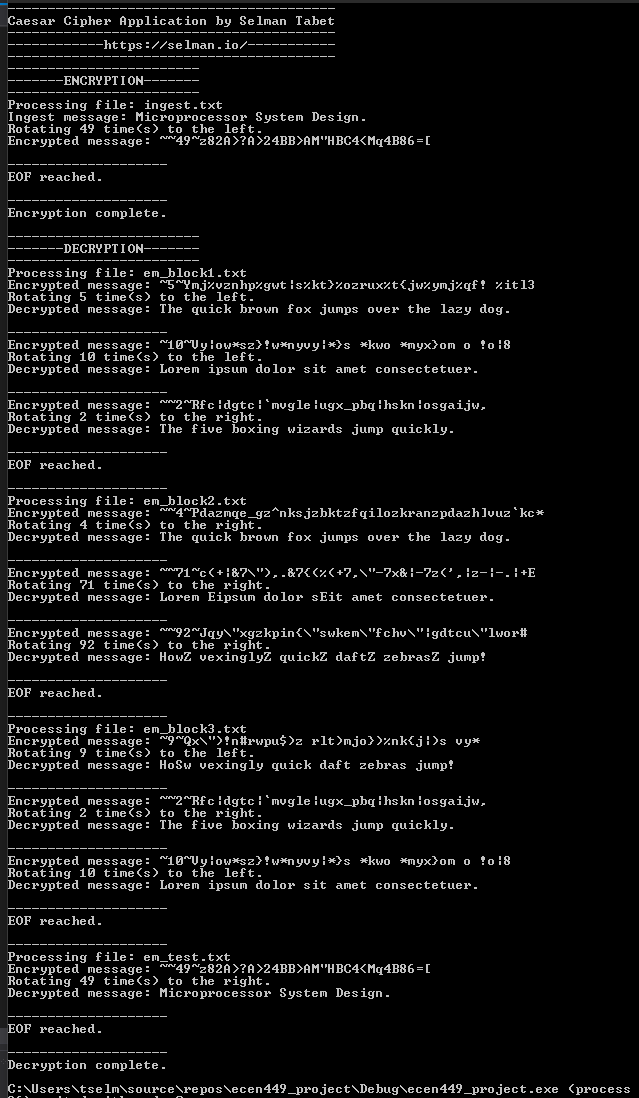
\includegraphics[scale=0.7]{Figures/Q1run.png}
\end{center}
\caption {Console program output.}
\label{fig:q1}
\end{figure}

\pagebreak

\section*{Pseudo-RNG Program}
\begin{minted}{cpp}
/* Selman Tabet (@selmantabet - https://selman.io/) - UIN 724009859
ECEN-449 Project - Part 2: Pseudo Random Number Generator (PRNG).

This program generates samples from a Gaussian distribution that is based on
two separate uniform distributionswith specified mean (mu) and standard
deviation (sigma). The program takes 2000 samples at a rate of 10Hz, and the
mean and standard deviation would be recomputed based on all samples collected.
The results would then be printed through the Serial port.
The error margin between the specified mean and the current calculated mean
are calculated and displayed as an integer value on the SPI 
interface (SPI LEDs on the board).

Developed using the Mbed IDE. Tested on an EA LPC4088 QuickStart Board. */

#include "mbed.h"
#include <stdio.h>
#include <stdlib.h>
#include <iostream>
#include <cmath>
#include <math.h>
#include <time.h>

Ticker tick; //Define ticker object
Serial pc(USBTX, USBRX); //Serial channel over HDK USB interface
SPI shifter(p5, p6, p7); //MOSI, MISO, SCLK
DigitalOut chip_select(p30); //Chip select

const int sample_size = 2000; //Can be dynamically adjusted per spec.
double samples[sample_size]; //Array of samples.

int counter = 0; //Keeps count for sigma calculations and for CLI print.
double sample; //Single sample.
double mean = 0; //Current mean value.
double std_deviation = 0; //Sigma (Standard Deviation AKA Variance^0.5)
int margin; //Integer percentage margin of error of the mean.

double rand_normal(double mu, double sigma) { //Box-Muller PRNG.

    /*Mersenne Twister engine (mt19937) is a more widely used PRNG (for good
    reasons) but the handout forces us to use rand() and Box-Muller. So here
    it is, for the sake of fulfilling the specified requirements.
    
    The implementation is based on the R. Knop revision of the method
    shown on the Wikipedia article linked in the handout. The z0 and z1
    formulae used here are available under the "Polar form" section
    of the Box-Muller Wikipedia article.*/
    
    static double z_1 = 0.0;
    static int z_1_cached = 0; //For temporarily storing z1 between calls.
    if (!z_1_cached)
    {
        double u, v, s; // u : x-component v : y-component  s : R^2 = u^2 + v^2
        do
        {
            u = 2.0*rand()/RAND_MAX - 1; //Uniform distribution 1.
            v = 2.0*rand()/RAND_MAX - 1; //Uniform distribution 2.

            s = u*u + v*v; //Polar form set expression.
        }
        while (s == 0.0 || s > 1.0); //Re-gen u,v pair if s-condition is false
        {
            double d = sqrt(-2.0*log(s)/s); //B-M intermediate.
            double z_0 = u*d;
            z_1 = v*d;
            double result = z_0*sigma + mu; //Scaling to defined parameters.
            z_1_cached = 1; //Use z1 on next call.
            return result;
        }
    }
    else
    {
        z_1_cached = 0; //Discard for pair regeneration on next call.
        return z_1*sigma + mu;
    }
}

void generate(){
    if (counter >= sample_size){
        pc.printf("Final mean: %f         Final standard deviation: %f\n",
        mean, std_deviation);
        exit(0);   
    }
    else {
        sample = rand_normal(10.0, 1.0); //Mean = 10, Sigma = 1.
        samples[counter] = sample;
        //Recompute mean and sigma.
        mean = ((mean * counter) + sample)/(counter + 1);
        double tmp = 0.0; //Squared-diff intermediate.
        for (int i = 0; i <= counter; i++){
            tmp += pow(abs(samples[i] - mean), 2.0); //Squared-diff summation.
        }
        counter++;
        std_deviation = sqrt(tmp / counter); //Final sigma calculation step.
        
        
        pc.printf("Sample #%i: %f    ( Mean: %f    Standard deviation: %f )\n",
        counter, sample, mean, std_deviation);
        
        margin = (int)((abs(10 - mean)*10) + 0.5); //Rounded via typecast.

        chip_select = 0; shifter.write(margin); chip_select = 1;
        
    }
}

int main(){
    chip_select = 0; //Select the device by setting chip select low
    shifter.write(0); //Clear LEDs
    chip_select = 1; //Deselect the device
    srand(time(NULL)); //Seed PRNG.
    tick.attach(&generate, 0.1); //Sampling rate set at 10Hz.
    while(1); //Run forever.
}
\end{minted}


The program generates a set number of samples from a Gaussian (AKA normal) distribution at a specified rate. The Gaussian distribution is formed using two uniform distributions followed by a Box-Muller transform and then scaled to the desired mean and standard deviation parameters. The \texttt{rand()} function is called to generate pairs that would eventually turn into the samples to be used in the program. Each resulting sample is stored in an array, and each sample number and its respective value is printed through the Serial port along with the updated mean and standard deviation of all the samples collected up to that point. The current mean is compared to the desired mean to give the margin of error as a rounded percentage integer. The integer is updated and loaded into the SPI LEDs on the board to reflect the current value at the sampling frequency.\pagebreak

The sampling process stops when the array is full, and the final mean and standard deviation values are printed. The larger the sample size (array size), the lower the margin of error is expected to be. Note that seeding to time does not work here as the program executes right after pushing the reset button and the only sense of time the board has is the time since reset, which is the same on every run. One way to resolve this is to seed the value to a chaotic powered source, like a plugged ADC (e.g. taking the least significant bit from an ADC that is configured at [\texttt{GND}-3.3V to 0-10k] 32 times to construct a 32-bit seed value). A different value can be seeded on every reset that way, bypassing the time-dependency issue. Figure \ref{fig:q2} shows the serial port output after a test run.

\begin{figure}[!ht]
\begin{center}
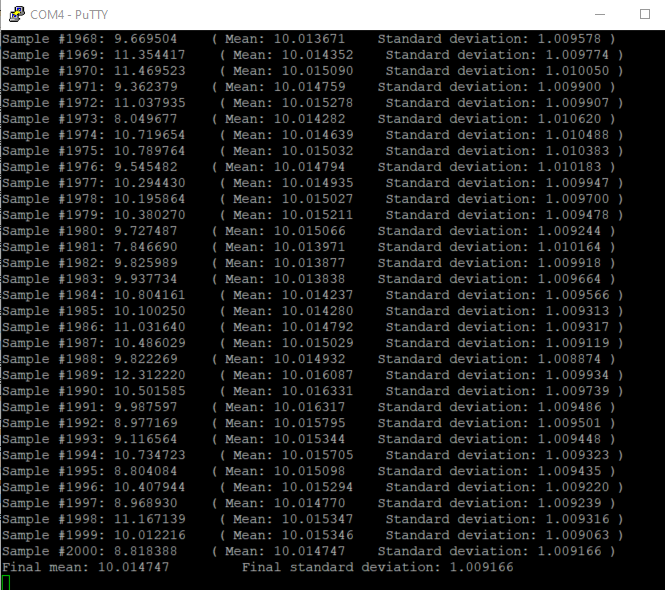
\includegraphics[scale=1.22]{Figures/Q2run.png}
\end{center}
\caption {PuTTY Terminal displaying the board's output through its Serial COM port.}
\label{fig:q2}
\end{figure}

\end{document}

